\documentclass{article}

\setlength{\parindent}{0pt}
\usepackage{graphicx}
\usepackage{hyperref}
\usepackage{amsmath}

\graphicspath{{../images/}}

\begin{document}

\section{H-2.1}

Bit stream: 11 00 10 00 11 11.

\subsection{Bipolar 8-ASK}

Bit stream: 110 010 001 111.

\subsubsection{Natural Mapping}
+5, -3, -5, +7

\subsubsection{Gray Mapping}
+1, -1, -5, +3
\subsection{16-QAM}

Bit stream: 1100 1000 1111.

\subsubsection{Natural Mapping}
+3-3j, +1-3j, +3+3j

\subsubsection{Gray Mapping}
+3+3j, +3-3j, +1+1j

\section{H-2.2}
In \autoref{fig:4qamnatural} and \autoref{fig:4qamgray} the 4-QAM constellations are shown for natural and gray mapping respectively.

\begin{figure}[h]
\centering
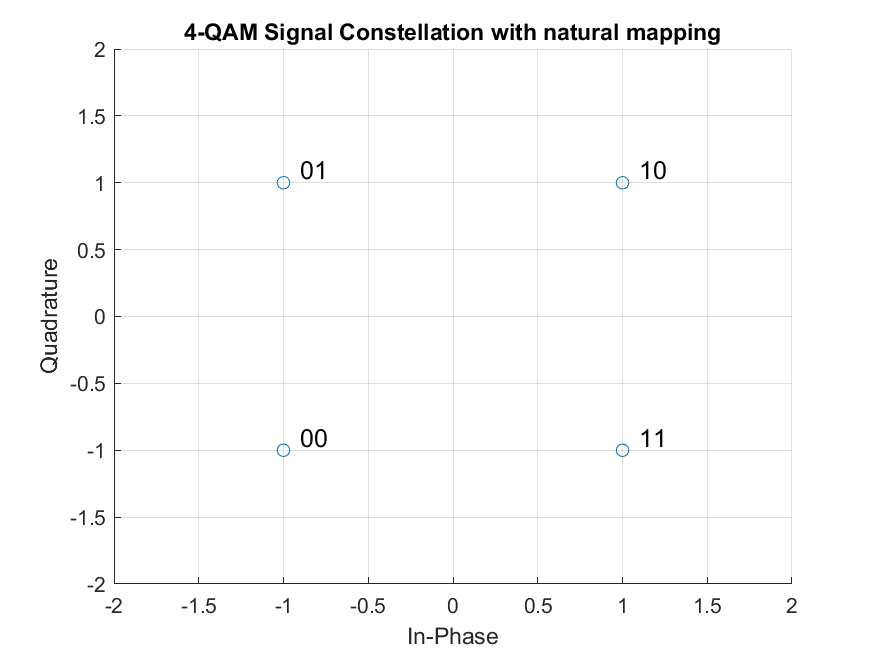
\includegraphics[width=0.6\textwidth]{4_QAM_natural.png}
\caption{4-QAM constellation with natural mapping}
\label{fig:4qamnatural}
\end{figure}

\begin{figure}[h]
\centering
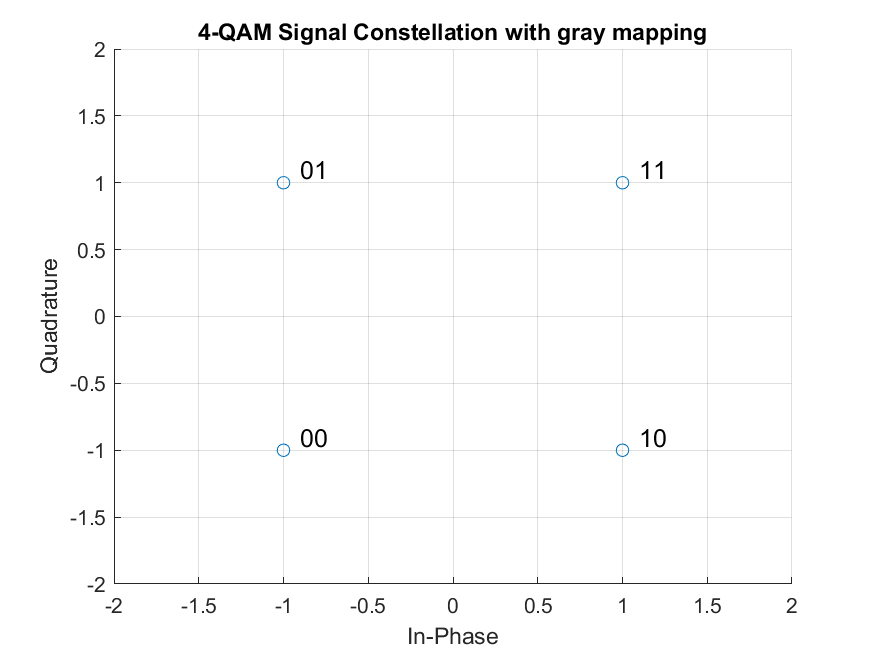
\includegraphics[width=0.6\textwidth]{4_QAM_gray.png}
\caption{4-QAM constellation with gray mapping}
\label{fig:4qamgray}
\end{figure}

Bitstream: 11 00 10 00 11 11

\subsection{Natural Mapping}
+1-1j, -1-1j, +1+1j, -1-1j, +1-1j, +1-1j

\subsection{Gray Mapping}
+1+1j, -1-1j, +1-1j, -1-1j, +1+1j, +1+1j

\section{H-2.3}

Bitstream: 01 010

Assuming gray mapping.

\subsection{4-QAM}
Symbol length is 2 bits, so we have 3 symbols. So we need to pad one 0 for the last symbol.

Zero padded bitstream: 01 01 0(0)

-1+1j, -1+1j, -1-1j

\subsection{8-ASK}
Symbol length is 3 bits, so we have 2 symbols. So we need to pad one 0 for the last symbol.

Zero padded bitstream: 010 10(0)

-1, +7

\subsection{16-QAM}
Symbol length is 4 bits, so we have 2 symbols. So we need to pad three 0 for the last symbol.

Zero padded bitstream: 0101 0(000)

-1+3j, -3-3j

\section{H-2.4}

\begin{equation}
s_{RF}(t) = \sqrt{2}Re\left\{s(t)e^{j2\pi f_{c}t}\right\}
\end{equation}

\begin{figure}[h]
\centering
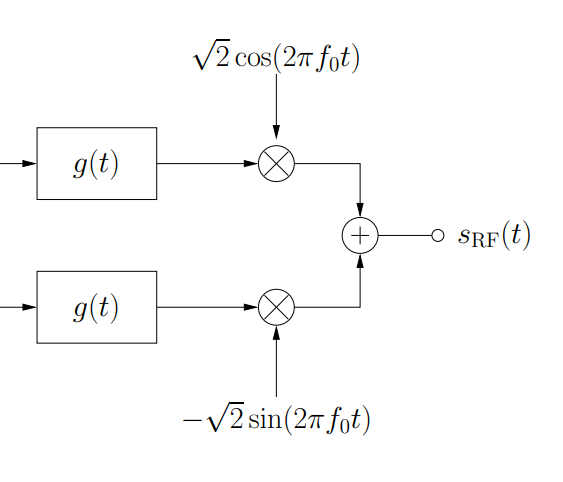
\includegraphics[width=0.6\textwidth]{modulation.png}
\caption{Modulation to carrier frequency}
\label{fig:modulation}
\end{figure}

\section{H-2.5}

$0\le t \le T$
\begin{align}
    s_{RF}(t) = \sqrt{2}Re\left\{s_1(t)e^{j2\pi f_{c}t}\right\} = \sqrt{2} Re\left\{3-5j[cos(2\pi f_{c}t) + j sin(2\pi f_{c}t)]\right\} = \\\nonumber
    = \sqrt{2}(3\cos(2\pi f_{c}t) + 5\sin(2\pi f_{c}t))
\end{align}

$T\le t \le 2T$
\begin{align}
    s_{RF}(t) = \sqrt{2}Re\left\{s_2(t)e^{j2\pi f_{c}t}\right\} = \sqrt{2} Re\left\{-1-1j[cos(2\pi f_{c}t) + j sin(2\pi f_{c}t)]\right\} = \\\nonumber
    = \sqrt{2}(-\cos(2\pi f_{c}t) + \sin(2\pi f_{c}t))
\end{align}

$2T\le t \le 3T$
\begin{align}
    s_{RF}(t) = \sqrt{2}Re\left\{s_3(t)e^{j2\pi f_{c}t}\right\} = \sqrt{2} Re\left\{7+3j[cos(2\pi f_{c}t) + j sin(2\pi f_{c}t)]\right\} = \\\nonumber
    = \sqrt{2}(7\cos(2\pi f_{c}t) - 3\sin(2\pi f_{c}t))
\end{align}

\section{H-2.6}

\begin{verbatim}
total = 0;

for i = 1:length(x)
    re = real(x(i));
    im = imag(x(i));
    pow = re^2 + im^2; 
    total = total + pow;
end

mean_power = total/length(x)
\end{verbatim}

\section{H-2.7}
\begin{equation}
    E_{b} = S_{e} T_{b} = S_{e} \frac{1}{f_{s} \log_{2}M}
\end{equation}

\section{H-2.8}

\begin{equation}
    P_N = 2 N_0/2 f_s
\end{equation}

\section{H-2.9}

\begin{figure}[h]
\centering
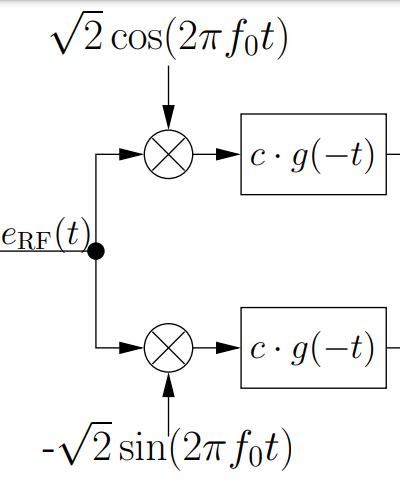
\includegraphics[width=0.6\textwidth]{demodulation.png}
\caption{Demodulation to carrier frequency}
\label{fig:demodulation}
\end{figure}

\section{H-2.10}

\begin{figure}[h]
\centering
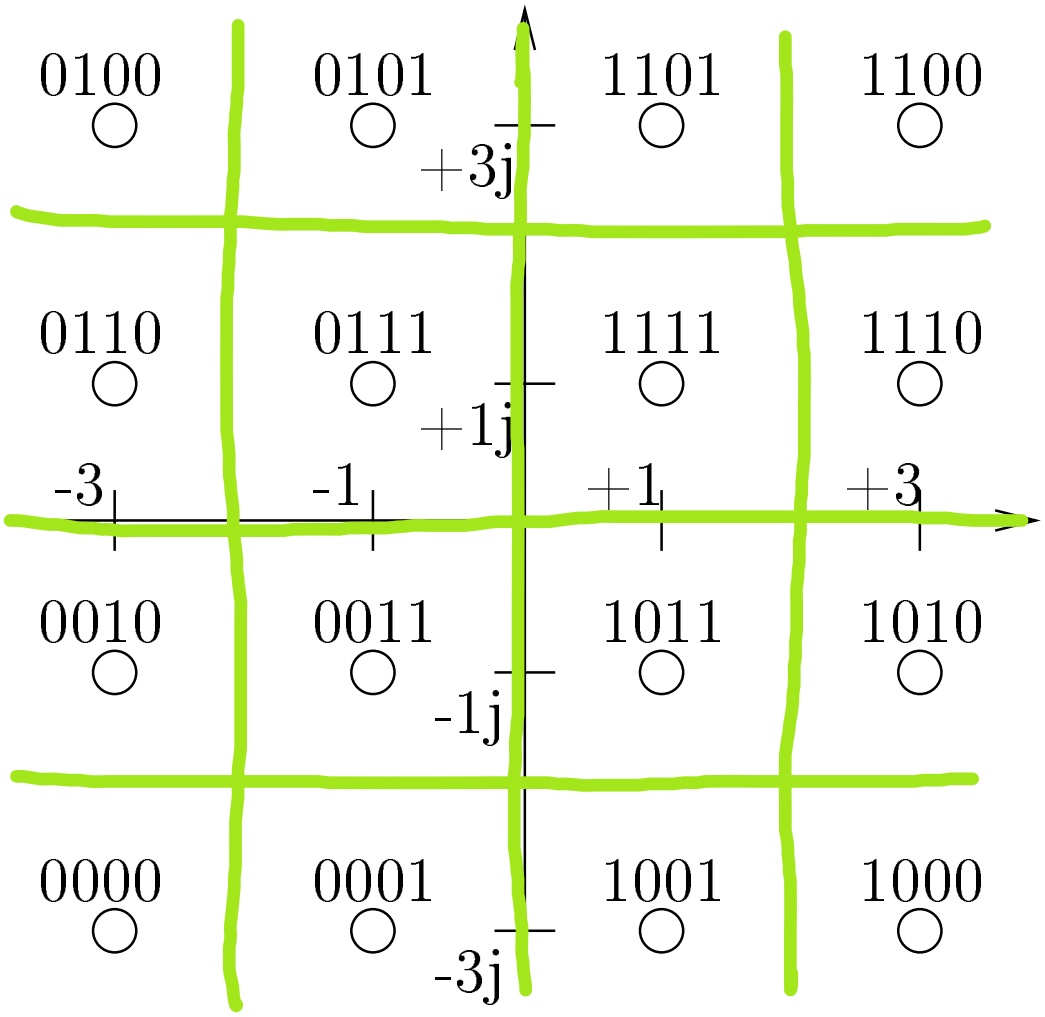
\includegraphics[width=0.6\textwidth]{16qam_decision.jpg}
\caption{16-QAM constallation with decision boundaries}
\label{fig:16qamdecision}
\end{figure}

\section{H-2.11 and H-2.12}
\subsection{Natural Mapping}
symbols: -3-1j, +3+1j, +1+3j
noise: +1.5-1.7j, +0.2+1.1j, -1.1+0.5j
symbolds with noise: -1.5-2.7j, +3.2+2.1j, -0.1+3.5j

estimated symbols: -1-3j, +3+3j, -1+3j
estimated bit sequence: 0100 1111 0111
origianl sequence:      0001 1110 1011
errors: 5
BER = 5/12 = 0.42

\subsection{Gray Mapping}

symbols: -1-3j, +3+1j, +1-1j
noise: +1.5-1.7j, +0.2+1.1j, -1.1+0.5j
symbolds with noise: +0.5-4.7j, +3.2+2.1j, -0.1-0.5j

estimated symbols: +1-3j, +3+3j, -1-1j
estimated bit sequence: 1001 1100 0011
origianl sequence:      0001 1110 1011
errors: 3
BER = 3/12 = 0.25

\subsection{Conclusion}
Gray mapping is better than natural mapping, as it has a lower error rate.
This is because, if an error happens with gray mapping, it is more likely that less bits are wrong, as the neighbors always differ by one bit.
This is not the case with natural mapping.

\section{H-2.13}
8-ASK

\subsection{Natural Mapping}

000, 001, 010, 011, 100, 101, 110, 111

Average bit error: $bit_{error} = \frac{1}{7} (1+2+1+3+1+2+1) = \frac{1}{7} 11 = \frac{11}{7}$

\subsection{Gray Mapping}

000, 001, 011, 010, 110, 111, 101, 100

Average bit error: 1

\section{H-2.14}

Count the number of wrong bits in the sequence (or how many need to be changed to get the origial sequence), and divide by the total number of bits.

\section{H-2.15}

For a confidence level (CL) of 95\%, the number of bits to test need to be $3 \times 10^6$, to have a BER lower than $10^{-6}$.
From \href{https://edadocs.software.keysight.com/kkbopen/how-do-i-measure-the-bit-error-rate-ber-to-a-given-confidence-level-on-the-j-bert-m8020a-and-the-m8040a-high-performance-bert-588276182.html}[

\begin{equation}
    N_{bits} = \frac{-\ln(1-CL)}{BER} = 3 \times 10^6
\end{equation}

\end{document}
